%=================
\chapter{Sprint 3}
%=================


%------------------------
\section{Sprint Planning}
%------------------------
For the third sprint we intend to implement the remanding requirements in the product backlog. We feel that the first and second sprint has resulted in a satisfying \gls{utility}, but it is still missing important functionality.

After two sprint iterations, we are still trying to improve our approach to \Gls{scrum}. Each sprint results in new ideas and better ways to do the process, and in this sprint we want everything to be correct and in the right order.\\
\\
There will be two major changes this sprint:
\begin {itemize}
\item We will have a complete planning meeting. The meeting should result in a good planning document, user stories for all the requirements, complete set of work items in the sprint backlog and a early understanding of the design. This approach will be differently from earlier sprints, where user stories was written in parallel with implementation. The user story should now be in place before the implementation, and the implementation should be based on the user story. This will make documenting the process easier, and will in turn give the advisors more documentation of what we are doing. Then we can receive valuable feedback from them.

\item In the sprint backlog we will have work items for every task that needs to be done throughout the sprint, including writing minutes, doing documentation, implementation and so on.  Assignment of responsibilities for items in the backlog should not be done at the planning meeting, we rather only give responsibility for one item for each team member at a time. The rest of the items will be unassigned. At each stand-up meeting we pick a task and must be done before the next meeting. This will ensure efficiency and the work done by others are easier to check and revise. It will give us a better work balance, as no team member can gap over too many tasks and leave none for the others.
\end{itemize}
We think that these changes will improve our work efficiency, and make sprint 3 the best one so far.


\subsection{Duration}
%-----------------------

The sprint started with the planning meeting the 19th of October and our work started the following day. The sprint duration is 14 days, and will end the 1st of November with a review meeting. 


\subsection{Sprint Goal}
%-----------------------
For the third sprint the team will update CSjark to version 0.3 which will extend the \gls{utility} so that it contains the complete functionality requested by the customer at this phase of the project. In this sprint we will pick all of the current requirements from the product backlog as all of the underlying functionality needed for them are already in place from the previous sprints. This means that we will also aim to create a draft of the final design of the system during the sprint.

The most important function that is going to be implemented in this sprint is being able to display packets from different originating platforms properly. This will be implemented by having every \gls{packet} contain a flag specifying their originating platform, and by having our \glspl{dissector} use this flag value to influence how it handles the data in the \gls{packet}.

\subsection{Back Log}
%--------------------
The work items concering features for this sprint are listed in Table \ref{tab:sprint3req}. These are covered by user stories and are about a fourth of the work in this sprint. See the timetable for the other work items.\\
Timetable for this sprint: Table \ref{tab:sprint3time}.\\

\begin{table}[!htb] \small \center
\caption{Sprint 3 Requirement Work Items \label{tab:sprint3req}}
\begin{tabularx}{\textwidth}{l X c c}
	\toprule
	& & \multicolumn{2}{c}{Hours} \\
	\cmidrule(r){3-4}
	User story & Req. and Description & Est. & Act. \\
	\midrule
	\textbf{Impl.} &  & \textbf{56} & \textbf{-} \\
	\hyperref[tab:req:stories7]{US29} & FR5-A: Flags specified for each platform &  5  & - \\
	\hyperref[tab:req:stories8]{US31} & FR5-C: \Gls{dissector} support both little and big \gls{endian} & 5  & - \\
	\hyperref[tab:req:stories8]{US32} & FR5-D: \Gls{dissector} support different sizes from flags & 12  & - \\
	\hyperref[tab:req:stories8]{US33} & FR3-C: Support WIN32, WIN64,\GLS{sparc} etc &  5  & - \\
	\hyperref[tab:req:stories7]{US29} & FR4-B: Configuration supports custom \Gls{lua} files & 6 & -\\
	\hyperref[tab:req:stories7]{US28} & FR2-C: Support \Gls{wireshark} filter and search on attributes &  3 & -\\
	\hyperref[tab:req:stories7]{US29} & FR5-B: \Glspl{dissector} support memory alignement & 4 & -\\
	\hyperref[tab:req:stories7]{US26} & FR1-D: Support members of type \gls{union} & 5  & -\\
	\hyperref[tab:req:stories7]{US27} & FR2-A add: Display a wildcard type for valid c types that \Gls{wireshark} has no support for & 3  & - \\
	\hyperref[tab:req:stories9]{US35} & FR4-D mod: Support specifying the ID of \glspl{dissector} (name and function) & 3  & - \\
	\hyperref[tab:req:stories9]{US39} & FR6-D: Don’t regenerate \glspl{dissector} & 1 & - \\
	\hyperref[tab:req:stories7]{US29} & FR2: Handle \Gls{lua} reserved definition names & 2 & - \\
	\addlinespace
	\textbf{Testing} &  & \textbf{19} & \textbf{-} \\
	 & FR4-B: Custom \Gls{lua} configuration & 2 & - \\
	 & FR5-C: \Glspl{dissector} support both little and big \gls{endian} & 1 & - \\
	 & FR5-D: \Glspl{dissector} support different sizes from flags & 2 & - \\
	 & FR3-C: Support WIN32, WIN64, \GLS{sparc} etc & 4 & - \\
	 & FR5-B: \Glspl{dissector} support memory alignement & 8 & - \\
	 & FR1-D: Support members of type \gls{union} & 1 & - \\
	 & FR2: Handle \Gls{lua} reserved definition names & 1 & - \\
	\addlinespace
	\textbf{Doc.} &  & \textbf{11} & \textbf{-} \\
	 & FR4-B: Custom \Gls{lua} configuration & 2 & - \\
	\hyperref[tab:req:stories8]{US34} & FR4-C: Support custom handling of specific data types & 2 & - \\
	\hyperref[tab:req:stories9]{US36} & FR5: User documentation for what platform that the \gls{utility} support & 3 & - \\
	\hyperref[tab:req:stories9]{US37} & FR5: Create developer manual from python docstrings (autodoc plugin) & 4 & - \\
	\addlinespace
	\textbf{Fixes} &  & \textbf{16} & \textbf{-} \\
	\midrule
	& Total: & 102 &  -\\
	\bottomrule
\end{tabularx}
\end{table}


\begin{table}[!htb] \small \center
\caption{Sprint 3 Timetable\label{tab:sprint3time}}
\begin{tabularx}{\textwidth}{X c c}
	\toprule
	& \multicolumn{2}{c}{Hours} \\
	\cmidrule(r){2-3}
	Description & Est. & Act. \\
	\midrule
	\textbf{Sprint planning} & \textbf{30} & \textbf{47.5} \\
	\addlinespace
	\textbf{Sprint 3 requirements} & \textbf{102} & \textbf{-} \\
	Implementation & 56 & - \\
	Testing & 19 & - \\
	User Documentation & 11 & - \\
	Fixes & 16 & - \\
	\addlinespace
	\textbf{Sprint review} & \textbf{20} & \textbf{-} \\
	\addlinespace
	\textbf{Sprint documentation} & \textbf{75} & \textbf{-} \\
	Sprint 1 document & 10 & -\\
	Sprint 2 document & 14 & - \\
	Sprint 3 document & 51 & - \\
	\addlinespace
	\textbf{Report work} & \textbf{42} & \textbf{-} \\
	User stories to LaTeX & 3 & 4\\
	Architecture update & 8 & -\\
	Glossaries and acronyms & 16 & -\\
	Requirement review & 15 & -\\
	Layout and correction & 15 & -\\
	\addlinespace
	\textbf{Lectures} & \textbf{21} & \textbf{14} \\
	\addlinespace
	\textbf{Meetings} & \textbf{57} & \textbf{-} \\
	Advisor meetings & 28 & - \\
	Customer meetings & 8 & - \\
	Stand-up meetings & 21 & - \\
	\textbf{Project management} & \textbf{20} & \textbf{-} \\
	\midrule
	Total: & 367 & - \\
	\bottomrule
\end{tabularx}
\end{table}



%----------------------
\section{System Design}
%----------------------
The system design defines the new modules and architecture that has to be in place to satisfy the specified requirements that we have included in the sprint 3 backlog. Most of the design are already done in earlier sprints; now we extend that and add some new elements.

\subsection{System overview}
%----------------------
Now that the \gls{utility} has both basic and advanced features, it is time to specialize and make support for environmental variables that can be found in Thales' source code. This basically include various platform specific support, \gls{endian} handling and minor technicalities. The latter one is vital for the customer in order for the \gls{utility} to be efficient and adequate.

\subsubsection{Platform specific support}
We know that the various platforms behave differently, and this must be supported by our \gls{utility}. The customer has mentioned at least three platforms that we have to support. As we emphasize extensibility and modifiability, it must also be expected that new platforms will be added or removed to the supported platforms in the future. Thereby we will try to make the set-up for support easily understandable.

We have decided that the platform definition will be a subpart of a flag-field in the structs header. To ensure modifiability we will assign a 16 bit field for this, giving the developers possibility to have 65536 unique platforms. From this we imagine that the platform flag can point to a dictionary which has the following information about the actual platform:
\begin{itemize}
\item Endianness
\item Length of fields
\item Memory alignment
\end{itemize}
All these three fields must be combined to enable the utility to generate a \gls{dissector} that will dissect the struct correctly.\\

The use of this information will be done in the config module, as you can see in the new class diagram MAKE REF.

\subsubsection{Dicitonary lookup}
Deciding how to implement handling of different platforms ended in a design draft seen in Figure \autoref{fig:platformhandling}. The \gls{dissector} module will make a dictionary lookup in the table of supported platforms. This table conatins all platforms that the \gls{utility} can make \glspl{dissector} for, and their information of how the \gls{dissector} shall be encoded to achieve correct handling of \gls{endianness}, length of fields and memory alignment.
We will start out by hardcoding this into the source code, but in the end we want to have this feed to the \gls{utility} through a configuration-file. This is the way the customer has envisioned it.  

%\begin{figure}[!htb]
%	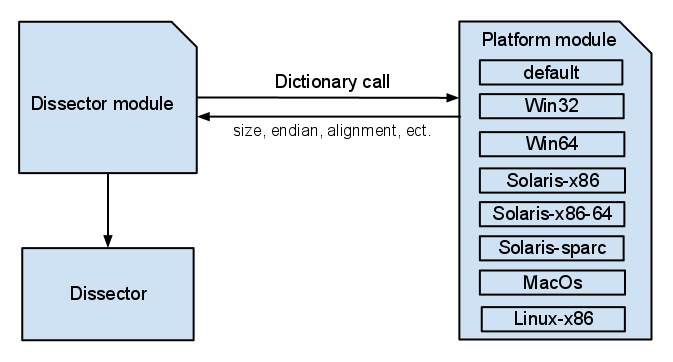
\includegraphics[width=\textwidth]{./sprints/img/platformhandling}
%	\caption{Platform handling\label{fig:platformhandling}}
%\end{figure}


\subsubsection{Endianness}
An important feature is the support for different endian handling. Endianness defines how the bits are ordered in the struct. It tells what bit is the most significant, and thereby the value that the bits represent. See the figure \ref{fig:endianness}.

\begin{figure}[!htb]
	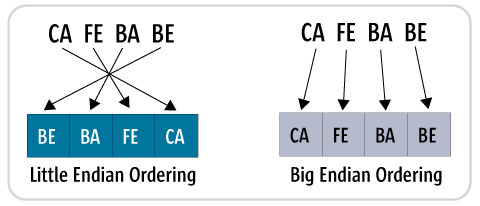
\includegraphics[width=\textwidth]{./sprints/img/endianness}
	\caption{Endianness\label{fig:endianness}}
\end{figure}

A design decision we made in the 
We know that Wireshark has support for reading both big- and little-endian. We understood that if the header could both be big and little endian, we would have problems, but Thales ensure us that headers always appear as small endian. So we need to dissect the data blob, which can be either big or small endian. By using the built-in reader support for endianness in Wireshark gave us much for free, but 


\subsubsection{Filter and search in \Gls{wireshark}}
The amount of data that are collected and dissected can be very large. The need for a filter and search mechanism is apparent. \Gls{wireshark} has this built-in, and the customer want the \gls{utility} to support it. To do that, we need to pass the abbrevation fields to Wireshark. These abbrevations will be generated by the dissector module and stored in the dissector made by the utility. Wireshark collects these when the actual dissector is used, and then a user will be able to search for them. In the design we have emphesized and assured us that the chosen abbrevations are descriptive, as the customer has stated it important in earlier customer meetings. 

\subsubsection{Technicalities}
Our design, and thereby implementation, will be influenced by Stig. He is a core developer for Wireshark and professional Python programmer. He points out things that we have done earlier that might not be efficient or not correct use. We have got some feedback on how elements should be passed to Wireshark.


\subsubsection{Batch processing}
The batch processing was implemented in the second sprint, but we need to modifiy it to make it able to process header-files even though it encounter some that it can not make dissectors for. 

%-----------------------
\section{Implementation}
%-----------------------
The main focus for this sprint was to support of different platforms. Several 
things are dependent on platform; \gls{endianness}, the memory allingment and sizes 
of data types. It is also possible that structs can be defined differnt for 
each platform. The \gls{utility} will generate different \glspl{dissector} for each 
platform. A \gls{dissector} this wil detect the platform and use the correct 
platform \gls{dissector}.

Support for the \gls{union} data type, finishing implementation of custom \Gls{lua} files 
and modification of functionallity implemented in the previous sprint was also 
done in this sprint.

\subsection{Specify Flags for Each Platform}
%-----------------------
It is necessary to specify flags for each platform to make it possible to 
correctly detect and display packages that wireshark captures. In wireshark 
the flags are used to tell which platform the \gls{packet} is sent from, so that 
the right \gls{dissector} is used to display the packets in \Gls{wireshark}. In the 
\gls{utility} the flag points to what kind of \gls{endianness}, how memory is aligned and 
the different sizes that is used for data types on the platform. These data 
are used to genereate a \gls{dissector} for the specific platform.

\subsection{Support Little and Big \Gls{endian}}
%-----------------------
Different platforms can order bytes in either little(left-to-right) or 
big(right-to-left) \gls{endian}. The \Gls{Windows} platform uses little \gls{endian}, and \GLS{sparc} 
uses big \gls{endian}. Since the \gls{utility} has to support both platforms, it was 
necessary to support handling of \gls{endianness}. The \Gls{lua} API in wireshark has 
functionallity to display data in both little and big \gls{endian}. Therefore the 
\gls{utility} has to read the specfied flag for the platform, and generate a \Gls{lua} 
\gls{dissector} that displays the data correctly for the given platform.

\subsection{Support Different Sizes from Flags}
%-----------------------
On different platforms, there can be different sizes on the data types. For 
example on windows a \emph{long double} is 8 bytes, and on sparc it is 16 
bytes. It is possible to specify sizes for data types for each platform. All 
these specifications is written in python code, and are easy to modify for the 
user of the system.

\subsection{Support Platform Specific Macros}
%-----------------------
All c complilers have predefined macros for different operating systems and 
processors. These macros are much used in code that need to be portabel for 
different platforms. When using these macros it is possible to create 
different struct members for each operating system, as shown in 
\autoref{code:predefmacro}, which will use different data types on each 
operating system. All platform specific macros are specified for each 
platform, so the dissector is generated correctly for each of the platforms. 
Currently all the platform specifications is done in python code.

\lstset{language=C,caption={Macros in C},label=code:predefmacro}
\lstinputlisting[language=C]{./sprints/code/predefmacro.h}

\subsection{Support Custom \Gls{lua} Files}
%-----------------------
Implementation of this feature started in sprint 2, and support for using 
conformance file to add lua code to correct places in the lua dissector was 
finished in this sprint. With the conformance file it is possible to add code 
before and after an member in both the definition and function part of the 
dissector. It also possible to replace the code for a member in both of these 
sections. In the example below there is written custom lua for a 
struct(temperature) with on integer member(celsius). In the conformance file 
in \autoref{code:customcnf} there added three lines of comments as a custom 
Lua code, that are going to be added to the Lua dissector. In 
\autoref{code:customlua} it is possible to see the custom Lua code that was 
added to the Lua dissector. The first comment is added after the member 
definition. The two other comments are added above and below the member in the 
function part of the Lua dissector.

\lstset{language=C,caption={Custom Lua conformance file},label=code:customcnf}
\lstinputlisting[language=C]{./sprints/code/custom.cnf}

\lstset{language=C,caption={Custom Lua dissector code},label=code:customlua}
\lstinputlisting[language=C]{./sprints/code/custom.lua}

\subsection{Support \Gls{wireshark} Filter and Search}
%-----------------------
Wireshark has a display filter, where it is possible to use packet filtering. 
Each field in our genereated dissectors has a abbrevation name that is 
connected to a struct. For each member of a struct, it is possible to filter 
for a value. An example is shown in \autoref{fig:wsfilter}, this shows a 
filtering for packets where Trondheim is equal to the member \emph{place} in 
the struct \emph{postcode}. 

\begin{figure}[ht]
	\center
	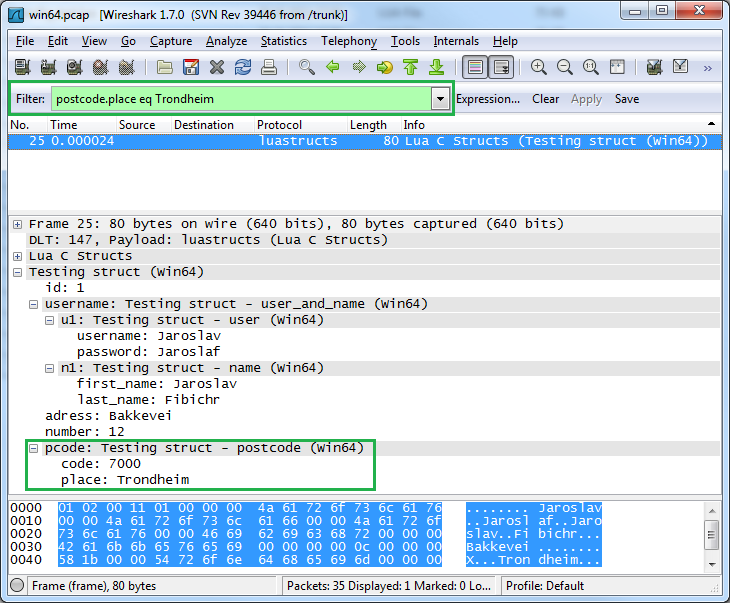
\includegraphics[width=\textwidth]{./sprints/img/wireshark_filter}
	\caption{Union type support\label{fig:wsfilter}}
\end{figure}

\subsection{Support Different Memory Alignment}
%-----------------------
TODO

\subsection{Support Union Type}
%-----------------------
The \gls{union} type is a variabel that can contain different data types with 
different sizes. The \gls{union} will allocated memory for the largest type defined 
in the \gls{union}. \autoref{code:union} shows an example on a header-file with an 
\gls{union} type. The compiler is responisble for keeping track of size and 
alignment requirements\cite[p.147]{Kerninghan1988} . Since there is not 
possible to find out which data type that is used in \Gls{wireshark}, the \gls{utility} 
has to genereate a \gls{dissector} that display the values for each data type. 
\autoref{fig:wsunion} displays the \gls{dissector} generated from the struct in 
\autoref{code:union}, this shows the \gls{union} with three members, all of them are 
listed with their values, in this case the float value is the correct one.

\begin{figure}[ht]
	\center
	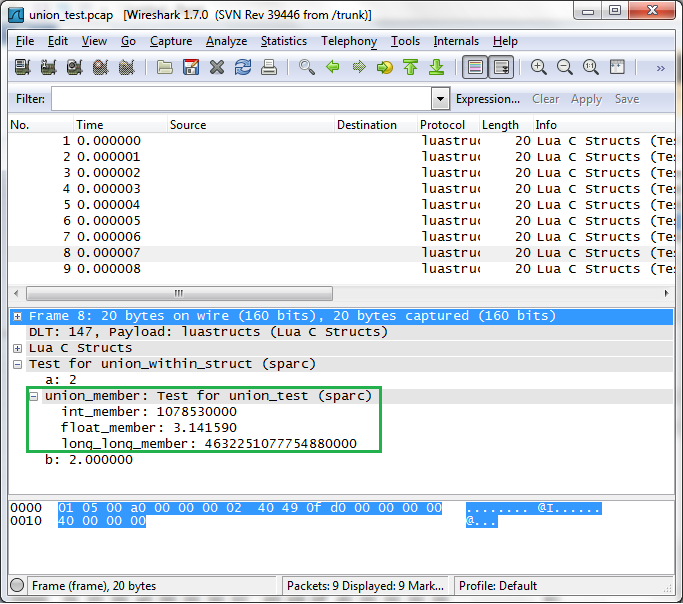
\includegraphics[width=\textwidth]{./sprints/img/wireshark_union}
	\caption{Union type support\label{fig:wsunion}}
\end{figure}

\lstset{language=C,caption={Union type},label=code:union}
\lstinputlisting[language=C]{./sprints/code/union.h}

\subsection{Display Types \Gls{wireshark} Do Not Support}
%-----------------------
TODO

\subsection{Support Specifying ID of \Glspl{dissector}}
%-----------------------
Specifying \gls{dissector} ID has been modified from sprint 2. The \gls{dissector} will 
still use the ID given in the configuration for a struct, if the struct is not 
given an ID in the configuration, then the ID for the struct will be set to 
\emph{NONE}. This is done to ensure that structs have an unique ID for their 
\gls{dissector}. Structs-in-structs member do not need an ID since they are called 
from the struct' by the \gls{dissector} name.

\subsection{Do Not Regenerate \glspl{dissector}}
%-----------------------
To increase the performance on generation of dissectors, dissectors that 
allready are genereated in batch mode, will only be generated once in a batch 
mode execution. This feature will be improved in the next sprint, so it only 
genereates dissectors in batch mode that are modified or new since the last 
batch run.

\subsection{Handle \Gls{lua} Reserved Keywords}
%-----------------------
\Gls{lua} has a list of reserved keywords, and some of these keywords are allowed in 
the C language. The \gls{utility} is able to support this under generation of \Gls{lua} 
code, when an identifier is a lua keyword, an underscore(\_) is added, so the 
identifier start with ''\_''.

\subsection{Support for Complex Arrays}
%-----------------------
Support for typedef was implemented in the previous sprint, in this sprint it 
has been improved to also support type definitions of complex arrays. Support 
for type definition of array is implemented, an example of such type 
definition in c is shown in \autoref{code:typedefarray}. Also support for 
arrays of enums, arrays, structs and pointers has been added.

\lstset{language=C,caption={Typedef of arrays},label=code:typedefarray}
\lstinputlisting[language=C]{./sprints/code/typedefarray.h}

%-----------------------
\section{Sprint Testing}
%-----------------------
During sprint 3 the team executed a total of 9 tests were run, but no additional testingfeatures were added during the sprint. Tests executed:

\begin{itemize}
	\item TID15 - Supporting batch mode of C header and configuration files \autoref{tab:sp3TID15}
	\item TID16 - Supporting custom \Gls{lua} configuration \autoref{tab:sp3TID16}
	\item TID17 - Supporting unions \autoref{tab:sp3TID17}
	\item TID18 - Supporting filter and search in wireshark \autoref{tab:sp3TID18}
	\item TID19 - Supporting WIN32, \_WIN64, \_SPARC etc \autoref{tab:sp3TID19}
	\item TID20 -  Supporting the use of flags specifying platforms to display member values correctly \autoref{tab:sp3TID20}
	\item TID21 - Supporting platforms with different \glspl{endian} \autoref{tab:sp3TID21}
	\item TID22 - Supporting alignments \autoref{tab:sp3TID22}
\end{itemize}

\begin{table}[!htb] \footnotesize \center
\caption{Supporting batch mode of C-headers and configuration files\label{tab:sp3TID15}}
\begin{tabular}{l l}
	\toprule
	Header & Description \\
	\midrule
	Description & Supporting batch mode of C header and configuration files \\
	Tester & Lars Solvoll Tønder \\
	Date & 28.10.2011 \\
	Result & Success\\
	\bottomrule
\end{tabular}
\end{table}

\begin{table}[!htb] \footnotesize \center
\caption{Supporting custom \Gls{lua} configuration\label{tab:sp3TID16}}
\begin{tabular}{l l}
	\toprule
	Header & Description \\
	\midrule
	Description & Supporting custom LUA configuration\\
	Tester & Lars Solvoll Tønder \\
	Date & 30.10.2011\\
	Result & success\\
	\bottomrule
\end{tabular}
\end{table}

\begin{table}[!htb] \footnotesize \center
\caption{Supporting unions\label{tab:sp3TID17}}
\begin{tabular}{l l}
	\toprule
	Header & Description \\
	\midrule
	Description & Supporting unions\\
	Tester & Lars Solvoll Tønder\\
	Date & 30.10.2011\\
	Result & success\\
	\bottomrule
\end{tabular}
\end{table}

\begin{table}[!htb] \footnotesize \center
\caption{Supporting filter and search in wireshark\label{tab:sp3TID18}}
\begin{tabular}{l l}
	\toprule
	Header & Description \\
	\midrule
	Description & Supporting filter and search in wireshark\\
	Tester & Lars Solvoll Tønder \\
	Date & 30.10.2011\\
	Result & success\\
	\bottomrule
\end{tabular}
\end{table}

\begin{table}[!htb] \footnotesize \center
\caption{Supporting WIN32, \_WIN64, \_\GLS{sparc} \label{tab:sp3TID19}}
\begin{tabular}{l l}
	\toprule
	Header & Description \\
	\midrule
	Description & Supporting WIN32, \_WIN64, \_\GLS{sparc} \\
	Tester & Lars Solvoll tønder\\
	Date & 30.10.2011\\
	Result & Failure. Most values were displayed correctly, but there were cases where the members and their values were different. Most notably in \gls{packet} 2 and 3 in the win64 and win32 \glspl{pcap-file} \\
	\bottomrule
\end{tabular}
\end{table}

\begin{table}[!htb] \footnotesize \center
\caption{Supporting the use of flags specifying platforms to display member values correctly \label{tab:sp3TID20}}
\begin{tabular}{l l}
	\toprule
	Header & Description \\
	\midrule
	Description & Supporting the use of flags specifying platforms to display member values correctly \\
	Tester & Lars Solvoll Tønder\\
	Date & 30.10.2011\\
	Result & Success\\
	\bottomrule
\end{tabular}
\end{table}

\begin{table}[!htb] \footnotesize \center
\caption{Supporting platforms with different \gls{endian} \label{tab:sp3TID21}}
\begin{tabular}{l l}
	\toprule
	Header & Description \\
	\midrule
	Description & Supporting platforms with different \gls{endian} \\
	Tester & Erik Bergersen\\
	Date & 31.10.2011\\
	Result & Success\\
	\bottomrule
\end{tabular}
\end{table}

\begin{table}[!htb] \footnotesize \center
\caption{Supporting alignments \label{tab:sp3TID22}}
\begin{tabular}{l l}
	\toprule
	Header & Description \\
	\midrule
	Description & Supporting alignments \\
	Tester & Lars Solvoll Tønder\\
	Date & 30.10.2011\\
	Result & Failure. All of the platforms that were used for testing were the same\\
	\bottomrule
\end{tabular}
\end{table}

\begin{table}[!htb] \footnotesize \center
\caption{Handling \Gls{lua} keywords \label{tab:sp3TID22}}
\begin{tabular}{l l}
	\toprule
	Header & Description \\
	\midrule
	Description & Handling \Gls{lua} keywords \\
	Tester & Lars Solvoll Tønder\\
	Date & 30.10.2011\\
	Result & Success\\
	\bottomrule
\end{tabular}
\end{table}

\subsection{Test Evaluation}

\subsubsection{Test Coverage}

%--------------------------
\section{Customer Feedback}
%--------------------------

\subsection{Pre-sprint}

The customer was satisfied with the functionality we implemented in sprint 2.
They feel that we are flexible and adapt well to their needs.
Some of the features from sprint 2 were postponed to sprint 3 because we needed additional feedback from the customer.
These include endianness and completing the handling of custom Lua files.

\subsubsection{New requirements}

We have assigned all the remaining requirements in the product backlog for this sprint.
If we are able to complete all the implementation tasks, the customer will provide us with more requirements for sprint 4.
The customer wants our utility to be as automatic as possible, and with as little configuration as possible. 
Additional requirements for sprint 4 will address optimization of the utility.

\subsection{During sprint}

In sprint 3 we again demonstrated our utility to the customer, and as a result we got some feedback on changes
and improvements we could make. The changes and additions are listed below.

\subsubsection{Wireshark, support of search and filter}

To support this the abbreviation field needs to be in place in our code

\subsubsection{Structs within structs}

The customer thought we displayed too much information in the info column in Wireshark,
 we should only display the name of the outer struct.

\subsubsection{Platforms}

We should not generate separate dissector files for the different platforms. It is much better if we have one protocol
with different functions for the different platforms, as this would not be such a performance hit.

\subsubsection{Flag values}

The customer said that our flag values were inconsistent, some flag values were platform names and some were operating
system names. They suggested using flags such as Solaris-x86, Solaris-SPARC, Win32 and Linux-x86.

\subsubsection{Testing of customer's header files}

The customer stressed the importance of our utility being able to run on the header files they have provided.
Once our utility is able to do this they can begin testing the utility on their own data.
We can expect to get a lot more feedback on the utility when they can test it themselves.


\subsection{The backlog and suggestions for sprint 4}

The customer was satisfied with the backlog for sprint 3.
They made several suggestions on features that could improve the utility, that we could implement in sprint 4.
These are listed below.

\subsubsection{Unitialized Memory}

It would be a nice if our utility were able to detect unitialized memory while debugging.
Different compilers use default patterns in members that are unitialized. If our utility could detect these patterns,
we could display the data in Wireshark with a warning that lets the user know that the data might have been unitialized.

\subsubsection{Dissector Ids}

The customer informed us that a struct could belong to several dissector IDs.
We should implement this by specifying a list of IDs instead of just a single one.

\subsubsection{Include dependency}

Christian describes that some structs may be included in other structs, which are resident in a different header file
not directly included in the  first, but both are included in a third header/source file. This creates a dependency which we must take
into consideration and implement in the utility.
TODO Rewrite this to english

\subsubsection{Specifying file name endings in batch mode}

The customer would like to be able to specify the file name endings of the files that are to be created dissectors for,
when running the utility in batch mode. The utility only needs to examine header files. The header files will have one or more known
file extensions, for example, .h and .hpp.

\subsubsection{Overall customer satisfaction}

In general the customer is satisfied with the progress we have made so far. Most of the requirements are
implemented or close to completion. When the utility is ready to be tested on their code, we can expect to receive
a lot of feedback on things we need to fix and improve.


















%--------------------------
\section{Sprint Evaluation}
%--------------------------


